\documentclass[12pt,a4paper]{article}
\usepackage[left=2.5cm,top=2.5cm,bottom=2.5cm,right=2.5cm]{geometry}
\usepackage{setspace}
\onehalfspacing
\usepackage[utf8]{inputenc}
\usepackage{graphicx}       % Add graphics capabilities
\usepackage{amsmath} 
        % Better maths support
 \usepackage{natbib}    % bibliography style
\setlength{\bibsep}{0.0pt}
\bibliographystyle{agsm}

\usepackage{amsmath}
\usepackage{amsfonts}
%\usepackage{mitpress}
\usepackage{amssymb}
\usepackage[USenglish]{babel}
%\usepackage{enumerate}
\usepackage{graphicx}
\usepackage[hidelinks]{hyperref}
\usepackage{booktabs}
\usepackage{siunitx}
\usepackage{threeparttable}
\usepackage{caption}
\usepackage{subcaption}
\usepackage{subfigure}
%\usepackage[document]{ragged2e}
\usepackage{outlines}
\usepackage{xcolor}
\usepackage{lscape}

\title{Expatriate Managers: Effects on Firm Performance\thanks{We thank Krisztián Fekete, Olivér Kiss, Szilárd Perédi, Bálint Szilágyi, András Vereckei, Rita Zágoni, and Gergő Závecz for excellent research assistance. The paper benefited from presentations at the Lunch Seminar of CEU, the London School of Economics, ETH Zürich, the University of Vienna, the 4th International Conference on Economics and Business Management (Cluj, Romania), the FIW conference in Vienna. This research was funded by the European Research Council (ERC Starting Grant agreement number 313164, ERC Advanced Grant agreement number 101097789) and by the National Research, Development and Innovation Office (OTKA contract number 143346 and Forefront Research Excellence Program contract number 144193). The views expressed in this paper are those of the authors and do not necessary reflect the official view of the European Union, the European Research Council, or the National Research, Development and Innovation Office. All errors are our own.}}

\author{Miklós Koren\thanks{Koren: Central European University, HUN-REN CERS Institute of Economics, CEPR and CESifo. Quellenstrasse 51, 1100 Wien, Austria. E-mail: korenm@ceu.edu.} \and Álmos Telegdy\thanks{Telegdy: Corvinus University of Budapest. 1091 Budapest, Fővám tér. 8. E-mail: almos.telegdy@uni-corvinus.hu}}

\date{June 2024}

\begin{document}

\maketitle
\thispagestyle{empty}

\begin{abstract}
\noindent Using a novel Hungarian dataset on firms and their Chief Executive Officers (CEOs), we estimate the impact of hiring expatriate CEOs. By examining foreign acquisitions where the new owner replaces the incumbent CEO with an expatriate or a local CEO, we address the selection into both acquisition and CEO hiring. Firms led by expatriate CEOs show 13 percent total factor productivity growth, 95 percent sales growth, and increase both exports and domestic sales. Hiring expatriate CEOs enhances firm performance in both international and domestic markets. Our findings suggest that expatriates have superior general management skills.
\end{abstract}

JEL Classification: F23 F61 L25

Keywords: Expatriate CEO, Foreign Acquisition, Firm performance, Hungary

\clearpage
\setcounter{page}{1}

%%%%%%%%%%%%%%%%%%%%%%
\section{Introduction}\label{sec: intro}
%%%%%%%%%%%%%%%%%%%%%%

Multinational enterprises (MNEs) often place expatriate managers in host countries to run their subsidiaries \citep{meyer2020managing}. Given the high wages and relocation costs of expatriate managers \citep{harvey2009expatriate}, there must be good reasons for the headquarters (HQ) to hire them.\footnote{Other downsides associated with expatriates include dealing with red tape and producing for the local markets \citep{tan2006multinational}. Expatriates can find it difficult  to adjust to the unfamiliar environment \citep{haslberger2013dimensions} which may cause underperformance \citep{collings2007changing} and premature resignation \citep{mcginley2008expatriate}.} Expatriates may have better overall management skills than locals because they are chosen from a larger group \citep{selmer2001expatriate}, may possess a better understanding of international markets and exporting \citep{piaskowska2014twice}, and may adopt modern management styles that lead to a more efficient organization of the subsidiary \citep{chang2012expatriate, fang2010multinational, meinen2022managers}.

Another argument for the widespread use of expatriate managers is that they possess skills that are specific to the MNE such as the knowledge of the internal processes of the firm \citep{collings2019global, harzing2001bears}. Expatriate managers may also serve as guardians of the headquarter's interests and thus solve the agency problems arising between the HQ and the subsidiary \citep{kostova2018understanding, o2000managing}. In addition, the practice of sending expatriate managers can also help strengthen their incentives \citep{grossman1986costs}. An expatriate assignment typically lasts for a few years, and managing a subsidiary may be a stepping stone for a higher managerial position in the headquarter. These career concerns can create high-powered incentives to the expatriate and diminish the agency problems arising between the acquirer and the target company.

While many reasons have been proposed why MNEs often choose expatriate managers, the causal effects of these managers on the target companies are still poorly understood. A major obstacle to constructing a causal estimate is that the headquarter considers a multitude of factors when deciding whether to send an expatriate manager, and many of these factors are unobservable to the researcher. As a consequence, firms receiving expatriate managers are not directly comparable to those under local management.\footnote{First, acquisitions \citep{bertrand2003enjoying} and foreign ownership \citep{Brown2006-rn} may alter firm behavior, which is hard to detach from the expatriate effect. Second, the expatriate effect is tied to the effect of managerial replacement. New managers tend to be more energetic as they are in need of proving their worthiness to the company. Moreover, it is the less productive firms that experience such replacements, which can introduce another bias in the estimated effect of expatriates \citep{denis1995performance}.}

We use novel administrative data on foreign-acquired firms in Hungary and their chief executive officers (CEOs) to obtain more credible evidence regarding the causal effect of bringing expatriate managers to the host country. Our setup has three distinctive features that help identification. First, our data source has universal coverage of all listed and unlisted corporations that were acquired by foreign owners between 1990 and 2019. Our sample will be dictated by our research design and not the convenience of observing particular types of firms. Second, the longitudinal nature of our data allows us to track firms before and after foreign takeover and replacement of management and to conduct event study analyses. Third, we observe the identity of the CEO of each corporation and we can use this information to precisely time the arrival of new CEOs and to classify them as expatriates, as we explain below.

Taken together, these three features of the data help us obtain a suitable comparison group to expatriate-managed firms. To minimize the bias arising from endogenous acquisitions, we limit our analysis to firms that were acquired by foreign owners in our sample. Furthermore, by focusing on firms that also replaced their management at the time of acquisition, we can control for the overall reorganization efforts of new management. Specifically, we compare the post-acquisition performance of firms acquired by foreigners where the CEO was replaced with an expatriate with those that replaced the incumbent CEO with a local one.\footnote{We study acquisitions where the acquirer is from a developed country. The reason for this is partly data driven: 84 percent of the foreign acquisitions in our are sample is from such countries. In addition, research shows that the distance in the grade of development between two countries is correlated with the foreign acquisition effect \citep{earle2018foreign}. Thus, we concentrate on the most prevalent segment of foreign acquisitions where the effects can be the highest.} We find that this narrow comparison group is, for most observables, indistinguishable from would-be expatriate firms before the acquisition. As we argue below, our method can credibly identify the effect of \emph{hiring} an expatriate CEO, which is the \emph{joint decision} of the owner and the CEO. Without more detailed data or experimental variation, we cannot distinguish whether the expatriate effects are due to decisions made by the owner or by the CEO.\footnote{In fact, we find it hard to conceive an experiment that credibly estimates this effect. Owners who agree to randomize the placement of their managers would likely be very different from the average owner, endangering the external validity of the experiment.}

To estimate what happens to firms when they get an expatriate CEO, we employ a new difference-in-differences method, which is based on \cite{callaway2021difference}. Essentially, we compare changes in outcomes for two groups of firms: \emph{both were acquired and changed the CEO in the same year}, but one group hired an expatriate while the other hired a local. The local-CEO group can thus serve as a control group for the expatriate-CEO group. This way we control for the potential bias arising due to staggered treatment and we also make sure that the control and treatment comparisons happen for the same treatment year and for the same time passed since the treatment. Existing difference-in-differences methods cannot do this as controls are not linked to treated units via a common treatment date.

We find that foreign acquisitions where the incumbent CEO was replaced by an expatriate CEO grow faster in the subsequent 5 years than those which end up with a local CEO, in terms of both capital and labor. They also increase total factor productivity (TFP), the volume of sales and the firm's export orientation (measured by the share of exports in total sales). Thus, firms managed by expatriates perform better along a multitude of important firm outcomes.

Our method rules out several potential sources of bias, such as the foreign acquisition effect, the CEO replacement effect, headquarter-subsidiary fixed effects, and the combined effect of the time of the treatment and the time passed since the treatment. The remaining threat to identification is that the new owner anticipates unobservable changes in business prospects and sends expatriate managers to subsidiaries with better prospects. Detailed event studies help alleviate these concerns: all measures of performance break sharply at the time when management is changed, and slowly moving inputs react sluggishly.\footnote{The sole exception is the export orientation of the company, where we cannot rule out a pre-existing trend. That is, expatriates may go to firms whose export share, though starting from the same level, is expected to grow faster. This behavior is consistent with a Grossman-Hart type acquisition, when the headquarter first trades with the firm and subsequently buys it up to solve the hold-up problem arising between the trading parties \citep{grossman1986costs}.} 

Are the skills of expatriate managers general or specific to the acquiring firm? To connect our results to the various hypotheses formulated in the literature, we compare different outcome variables on two subsamples: tradable and nontradable sectors.\footnote{This classification is highly correlated with vertical and horizontal integration.} Better \emph{general management skills} would increase both the productivity and the scale of the firm, irrespective of the sector and the market served (international of domestic). A tighter \emph{integration into international markets} would imply a disproportionate expansion of export revenue, and smaller expatriate effects in nontradable sectors and domestic sales. And a stronger \emph{alignment with the owner's interest} would be associated both with higher exports and faster capital investments, but the high-powered incentives of the CEO may also boost productivity and domestic sales.

We find large positive domestic sales growth for expatriate CEOs. The overall expansion in employment and sales, as well as the improvement in productivity are larger in nontradable sectors, suggesting that the general management skills of expatriates are much better than that of locals. By contrast, export effects are small, downplaying the importance of the export experience mechanism. The sharp increase in the rate of investment for expatriate-managed firms is consistent with the owner's guardian mechanism. In summary, while none of the three main mechanisms are rejected in the data, the strongest evidence points to better general management skills of expatriates.

Our research is primarily related to the emerging body of literature examining the impacts of expatriate managers on firm performance. The subsidiaries of Japanese MNEs with expatriate managers have superior performance only in developed, but not in developing countries \citep{ando2014effect} and this effect declines with the cultural distance from the host country \citep{gong2003subsidiary}. In the United Kingdom,  MNEs with expatriate managers do not fare better than other firms, but domestic firms do \citep{exadaktylos2024talents}. Finally, the affiliates of South Korean MNEs experience a faster productivity increase if they are staffed with Korean managers \citep{cho2018knowledge}. Two of these papers use data that allow reducing the bias arising from the joint decision of takeover and the identity of the manager: \cite{exadaktylos2024talents} perform propensity score matching between firms with and without expatriate managers and \cite{cho2018knowledge} employ system GMM.

Second, our research is connected to the literature which emphasizes the significance of CEOs in shaping firm behavior. This literature demonstrates that CEOs are not easily substitutable with one another \citep{bennedsen2020ceos, huber2021discrimination}, that their managing styles shape firm behavior \citep{bandiera2020ceo}, that good training increases firm performance \citep{Bloom2012-ek,giorcelli2019long}, and that personality traits also matter \citep{kaplan2022ceo}. We add a new, observable, trait to this literature: whether the CEO is local or foreign, and find that it is strongly correlated with general management skills.

%% observable traits

%%%%%%%%%%%%%%%%%%%%%%%%%%%%%%%%%%%%%%%%%%%%
\section{Data Construction}\label{sec: data}
%%%%%%%%%%%%%%%%%%%%%%%%%%%%%%%%%%%%%%%%%%%%

\subsection{Data on CEOs}

Data on managers originates from an administrative dataset compiled and maintained by the Hungarian Corporate Court \citep{cegjegyzek}. According to Hungarian Corporate Law \citep{cegtv}, businesses have to maintain accurate public records about their corporation at county courts. Among other relevant information such as owners and business locations, companies must register all individuals who can represent the company in legal or business matters (``representatives"). Such representatives include CEOs, other managers and directors of the company, but also legal counsels and lower-ranked employees with signatory rights.\footnote{In rare cases, such as when the firm is in bankruptcy proceedings, the representative may be a legal entity. We exclude these cases.}

Electronic court records start in 1992 and the last year we use is 2019. The data also contain the starting date of service for the representatives even if this date is before 1992, which allows extending the time span of the data. In this subsection we outline the procedures employed to construct an operational dataset from the raw data.

Information on representatives includes a number of personal identifiers, such as name, mother's name, birth date, and home address. Before 2010, the data contains no numerical identifier uniquely identifying the person. Court records constitute a \emph{temporal database}, which means that each entry has an effective date interval (see Appendix Table \ref{table:rawdata} for a hypothetical example). Over the decades covered by our sample, new entries are added not only at times of hiring, firing and change in corporate position, but also when any individual identifier changes or when the reporting requirements change. For example, if a representative moves to a new address, she gets a new entry. An additional complication is that effective dates are not always filled in. 

Our first task was to identify which of the predominantly text-based records referred to the same person as a company representative. This entity resolution enabled us to assign a unique identifier to each person and to track them over time within a firm and across firms. We then had to solve three problems to obtain our analysis dataset: (1) setting the period of service in a given position, (2) identifying CEOs, and (3) identifying expatriates.

\paragraph{Period of service.} We set the starting and ending dates of each manager in a given position by filling in missing dates from the available neighboring records. Corporate Court records are entered sequentially, so we can set bounds on missing starting and ending dates. For example, if a manager is recorded to leave, after which a new manager is registered without a starting date, we impute her starting date as the day on which the previous manager left. At the edges of the list, we use information about the firm's life cycle: if the firm was established in June 1993, we can assume its first representative also started then, even if this is not recorded in the data.

As the financial information is reported annually, there is no reason to use within-year changes of the management. We create an annual panel of managers by keeping the records which include June 21 (so the start date of the position is before, and the end date later than June 21 of the given year). 

\paragraph{CEOs.} Firm representatives always include the CEO, but can also include lower ranked managers and other employees with signatory rights. The precise occupation of the manager is not recorded in a standardized way. Instead, there are many expressions for the same occupation. Chief executives (``managing directors'') should, in principle, always be flagged as such. If we have this information, we use it. For firms that do not report a CEO in a given period, we proceed as follows. 

If there are three or fewer representatives at the firm in a given year, we assume that all of them are CEOs. If there are still no CEOs at the firm (because there were more than three representatives), but one of the representatives was a CEO in the past, we set this person to be the CEO. In our final sample, 76 percent of firms have one CEO in the year before foreign acquisition, 17 percent have two, the rest have three or more. We drop all firms with 15 or more CEOs throughout the sample period. Firms led by co-CEOs may be real, but can also be the result of our data cleaning.\footnote{Research shows that this leadership structure is uncommon, but existent in public firms in the US \citep{krause2015s}, but we did not find any study showing the prevalence of co-CEOs among private firms. As our estimation method hinges upon the identification of new hiring and expatriate CEOs and not the number of executives, this potential data deficiency does not affect our results.}  

%% . xt2treatments n_ceo, pre(4) post(4) treatment(has_expat_ceo ) control(local_ceo )
%%
%%Panel variable: frame_id_numeric (unbalanced)
 %%Time variable: year, 1986 to 2019, but with gaps
         %%Delta: 1 unit
%%
%%Event study relative to -1              Number of obs = 12,714
%%
%%------------------------------------------------------------------------------
%%       n_ceo |       ATET   Std. err.      z    P>|z|     [95% conf. interval]
%%-------------+----------------------------------------------------------------
%%          -4 |  -.0491853   .0443128    -1.11   0.267    -.1360369    .0376662
%%          -3 |  -.0136249   .0304694    -0.45   0.655    -.0733439    .0460941
%%          -2 |   .0132974   .0185691     0.72   0.474    -.0230974    .0496922
%%          -1 |          0  (omitted)
%%           0 |   .6370581   .0544978    11.69   0.000     .5302444    .7438719
%%           1 |   .6228139   .0618636    10.07   0.000     .5015634    .7440643
%%           2 |   .6498526   .0711452     9.13   0.000     .5104105    .7892946
%%           3 |   .6349408   .0751226     8.45   0.000     .4877032    .7821784
%%           4 |   .6403844   .0754551     8.49   0.000     .4924952    .7882736
%%------------------------------------------------------------------------------


In our analysis, we are interested in the replacement of CEOs by the new foreign owner. In the case of multiple CEOs, we classify an event as ``CEO change'' whenever a new CEO was hired, irrespective of what happened to the other CEOs.\footnote{Including CEO firings in the definition of ``CEO change'' does not affect our results.}

\paragraph{Expatriates.} Finally, we classify whether the CEO is local or foreign (``expatriate'') with the help of both the name of the representative and her first recorded home address. 

Several peculiarities of Hungarian names help us differentiate local managers from expatriates. First, Hungarian law restricts the selection of first names for its citizens to a predetermined list \citep{anyakonyv,nevlista}. If the given name of a person was on the list, we considered her Hungarian.\footnote{If parents belong to an ethnic minority, they may choose names from a different list. Since Hungary is ethnically fairly homogeneous and parents belonging to ethnic minority groups often choose Hungarian names.} Second, Hungarian follows the Eastern name order (placing the family name first and the given names last) so even with internationalized given names, we can distinguish the Hungarian version. Third, many names have accents or otherwise different spelling from international variants, further aiding differentiation. For example, ``Richter Éva'' would be classified as a Hungarian name, because the last word is an approved Hungarian given name and the name order is Eastern. At the same time, ``Eva Richter'' would be classified as a foreign name. After the visual inspection of several hundred entries coded as Hungarian or foreign individuals, we are confident in the quality of this segmentation algorithm.

The use of the home address of the CEO poses both an opportunity and a challenge. The opportunity is that if the home address of a CEO is foreign, we can also classify the sending country by its overall level of development. We can thus limit the analysis to countries that are both significant investors in Hungary and also technologically advanced.\footnote{We included Austria, Belgium, Canada, Denmark, France, Germany, Ireland, Israel, Italy, Japan, Korea, the Netherlands, Norway, Spain, Sweden, Switzerland, the United Kingdom, and the United States as sending countries. Together, they account for 84 percent of expatriate CEOs in the foreign acquisition sample.} The challenge is that CEOs often move to the place of their company, and we would only observe their Hungarian address. We have reviewed the names of all 133 CEOs in our sample that were classified as having a foreign name and a Hungarian address. We found 14 CEOs to be Hungarian (misclassified due to unusual given names or misspellings), 78 to have names in languages of our sending countries (German, English and Italian being the most common). The remaining 41 CEOs with names from other countries were excluded.


\subsection{Data on companies and sample construction}

\paragraph{Company data.} We use the financial statements of the population of Hungarian double-entry book keeping firms for the period between 1992 and 2019, as well as several other variables -- employment, the location and main activity of the firm and the share capital owned by domestic and foreign entities \citep{merleg}.\footnote{Up to 2002, there is a significant number of small firms that did not engage in double-entry book keeping while in the latter period the number of such firms radically declines. Single-entry book keeping firms are predominantly very small and would not be included in our data anyway.} We augment the company data with balance sheet information for the period between 1986-1991. These data are recorded according to the Socialist book keeping, but all the key variables used in this analysis are included (ownership only for 1990 and 1991, but there were very few foreign-owned companies in the eighties).

We transform ownership shares into dummy variables. We define a firm as foreign-owned if the majority of its share capital is owned by foreigners.\footnote{Other thresholds, such as 10 percent, lead to a very similar number of foreign firms.} We also consider a firm as foreign-owned if it is owned by a foreign subsidiary registered in Hungary.

We proxy vertical and horizontal integration with the sector of the firm: if the firm belongs to a tradable sector, the purpose of the acquisition was probably vertical integration while in the case of nontradable sector, horizontal integration. We define tradable sectors based on the NACE code of the firm in the pre-acquisition year.\footnote{The following sectors are coded as tradable (the others are nontradable): agriculture, mining, manufacturing, energy, water transport, air transport, warehousing and support activities for transportation, publishing, video production, broadcasting, telecommunications, computer programming, information service, legal and accounting, activities of head offices, engineering, research and development, advertising, other professional activities.}

\paragraph{Final sample.} We link the managerial data to the financial statements with the help of the tax identifier of the company. This eight-digit identifier can change during reorganizations, but we can link the same firm over time even if they changed their identifier.

We are interested in domestic firms that were acquired by foreign investors and the acquisition was accompanied with a CEO replacement. If the firm was later divested, we drop the years after the divestment.\footnote{If the firm underwent more than one foreign acquisition during the sample period, we drop the entire firm.} This makes foreign acquisition a permanent treatment in our sample.  

Close to acquisition time most, but not all, CEO replacements took place in the same year with the acquisition itself. If the expatriate CEO arrived a year ``early'' or a year ``late,'' relative to the time of acquisition, we adjusted the time of acquisition to match the arrival of the new CEO. In other words, we believe CEO starting dates to be more accurate than reported changes in foreign ownership. We drop firms where the expatriate manager arrived two or more years before the ownership change. If an expatriate CEO was later replaced with a local CEO, we drop the latter years. We allow, however, for expat-to-expat and local-to-local transitions. 

We keep only firms with an average employment of at least 10 employees for the years included in the sample, as foreign ownership and expatriate managers are scarce among very small firms. We drop firms in financial services, those that have more than 15 CEOs during the studied period and we only use firm-years with non-missing data for sales, employment, the value of tangible assets and material costs. To concentrate on the period around the acquisition, we trim the data and keep a time window of 4 years before and 5 years after the acquisition.

The final sample has 1,995 firms, out of which 1,522 got a local and 473 an expatriate CEO at the time of the acquisition. The number of firm-years is 12,714. The average number of pre- and post-acquisition years is 3.4 and 4.2, respectively. The mean and median number of employees in our sample is 93 and 30.\footnote{During the nineties, the main vehicle of FDI was the privatization of state-owned enterprises. In our data, 12 percent (234 firms) of the acquisitions are privatization transactions, out of which 215 firms got a local and 19 an expatriate CEO. Exclusion of the privatization transactions from the analysis leads to similar conclusions, with the expatriate effect on capital being somewhat smaller, and on total and domestic sales larger.}

On the resulting sample, we estimate a Cobb--Douglas production function to recover the total factor productivity (TFP) of firms. The dependent variable is the value of sales and the explanatory variables the book value of capital, the number of employees and the value of material costs (all logged). We estimate this regression using ordinary least squares for industrial and service firms separately, and control for 2-digit-industry-year interaction. The residual resulting from these regressions is a measure of the TFP of the company.\footnote{We estimate TFP separately from the expatriate CEO effect as our method does not allow the inclusion of control variables in the regression.}

\subsection{Descriptive statistics} 

Table \ref{tab:desc} presents the means and standard deviations of several variables for firms with a local and expatriate CEO in the year before acquisition. Expatriate CEOs are more likely to be placed in the tradable sector. They tend to manage larger firms than locals by both employment and the value of tangible assets, but they have lower sales. For example, the average number of employees is 85 in firms that would get a local CEO and 134 in those with an expatriate CEO. Expatriate led companies are more capital intensive before acquisition and they are also more export oriented as the share of exports in total sales is 22 percent, 10 percentage points larger than of firms that obtain a local CEO. Finally, expatriates get firms that are less productive.

These differences mostly disappear when we consider all these factors together. In Table \ref{tab:select} we present the estimated coefficients of a linear probability model with the dependent variable indicating expatriate CEO and explanatory variables being the firm characteristics before acquisition: employment size, capital intensity, productivity and export share. In Column 1 we also add a dummy for tradable sectors and another for early acquisition (before 2000) while in the second column we replace these two dummies with a full set of 2-digit industry-year fixed effects and we also control for the year of acquisition. Expatriate CEOs are more prevalent in tradable sectors and they came in larger numbers in the early period. The other variables are associated with coefficients that are small in magnitude and have a large standard error. In Column 2, where we control for industry-year interactions and the time of acquisition (as we do in the regressions), the size of the coefficients declines further. For example, the firms situated at the 75th percentile in the distribution of export share has a higher chance of getting an expatriate CEO of 0.006 relative to the firm situated at the 25th percentile. Taken together, these regressions suggests that observable factors do not play an important role in the choice of the type of CEO after acquisition.


%%%%%%%%%%%%%%%%%%%%%%%%%%%%%%%%%%%%%%%%%%%%%%%%%%%%%%%%
\section{Estimation Method and Results}\label{sec: meth}
%%%%%%%%%%%%%%%%%%%%%%%%%%%%%%%%%%%%%%%%%%%%%%%%%%%%%%%%

\subsection{Methodology}

Take the following model for outcome variable $Y$ in year $t$ at firm $i$ which was acquired in year $g$,\footnote{For each $g$, we add 4 pre- and 5 post-treatment years, $t=g-4,...,g+4$.}
\begin{equation}\label{eq:reg}
    Y_{igt} = \alpha_i + \nu_{gt} + \gamma_{gt}\times \text{Expat}_i + \varepsilon_{igt}.
\end{equation}
Note that $g$ is also defined for firms that received a local CEO instead of an expatriate (``control firms''). The outcome variable is assumed to depend on a firm fixed effect $\alpha_i$, a fixed effect for the interaction of treatment time and calendar time $\nu_{gt}$, and a treatment effect for firms run by expatriate managers, the variable of interest.

We follow \cite{callaway2021difference} and allow for heterogeneity in mean outcomes not only over calendar time $t$, but also for different treatment cohorts $g$. Business cycles and inflation can introduce heterogeneity in calendar time. Differences in economic policy stance towards foreign acquisitions can introduce heterogeneity in treatment cohort. Because we include fixed effect $\nu_{gt}$ for each combination of treatment cohort and calendar time, we are effectively comparing firms with an expatriate manager to other firms in the same year with a local manager, that were \emph{acquired at the same time}. The identification assumption is that $\varepsilon_{gt}$ is orthogonal to treatment status for all $g$ and $t$.

As the time series of firms are as long as 34 years and the treatment of expatriate CEO is staggered in time, traditional OLS estimates of a two-way fixed effects model will produce biased results \citep{de2020two}. To estimate the expatriate CEO effect on firm behavior, we develop a new difference-in-differences method building on \cite{callaway2021difference}. Our method proceeds in three steps. First we compare all outcome variables of a firm to their level in the pre-acquisition year (the ``first difference''). Second, we estimate mean differences between expat-managed and local-managed firms within each cohort (the ``second difference''). Third, we average these treatment effects across all cohorts with appropriate positive weights.\footnote{The method is an extension of \cite{callaway2021difference} to two treatments, where one treatment can be used as a control group for the other. Indeed, if we estimate two separate treatment effects $\gamma_{\text{Expat},gt}$ and $\gamma_{\text{Local},gt}$ relative to a common control group using \cite{callaway2021difference}, the difference $\gamma_{\text{Expat},gt}-\gamma_{\text{Local},gt}$ is numerically identical to our estimator for all $g$ and $t$.}

Perhaps it is useful to compare our method to that of \cite{callaway2021difference}. Typical applications do not specify $g$ for the control group, they compare treated firms with controls in the same $t$, but not in the same $g$, and one untreated firm-year can serve as control for treated firms with different $g$s. Our method is more strict in the sense that we dedicate a special control group for each group treated in $g$: those firms that are also treated in $g$, but with a different treatment. In addition, we compare the evolution of $Y$ between treated and control groups for the same time distance relative to the treatment.

We estimate this model as follows. We first we express the outcome variable relative to the year before foreign acquisition, $t=g-1$,
\begin{equation}\label{eq:reg2}
    \tilde Y_{igt} = \nu_{gt} + \gamma_{gt}\times \text{Expat}_i + \tilde\varepsilon_{igt},
\end{equation}
where $\tilde Y_{igt} = Y_{igt} - Y_{ig,g-1}$ and we have normalized the fixed effects and the treatments effects to zero when $t=g-1$. This step removes the firm fixed effects. 

We then use regular fixed effects estimation \citep[version 6.12.5]{reghdfe} to recover estimates $\hat\nu_{gt}$ and $\hat\gamma_{gt}$. Note that $\hat\nu_{gt}$ is simply the mean outcome difference, relative to period $g-1$, among firms that were acquired in the same period $g$ but did \emph{not} receive an expatriate manager. 

Similarly, $\hat\gamma_{gt}$ is simply the mean difference in (differenced) outcome between treated and control firms. Instead of reporting the mean difference for each cohort $g$ and year $t$, we compute two kinds of weighted averages, as implemented in the Stata module \texttt{xt2treatments} \cite[version 0.8.4]{xt2treatments}. Average treatment effect on the treated is defined as the average of post-treatment differences minus pre-treatment differences between the treatment and the control group,
\begin{equation}
    \hat\gamma_{\text{ATT}} := \frac{\sum_{g,t: t\ge g}\omega_{gt}\hat \gamma_{gt}}{\sum_{g,t: t\ge g}\omega_{gt}} - 
    \frac{\sum_{g,t: t < g}\omega_{gt}\hat \gamma_{gt}}{\sum_{g,t: t < g}\omega_{gt}}.
\end{equation}
We use the weight $\omega_{gt} = n_{1gt} n_{0gt}/(n_{1gt}+n_{0gt})$, where $n_{1gt}$ is the number of treated firms that were acquired in year $g$ and have non-missing data in year $t$, and $n_{0gt}$ is the number of control firms in this same group. This weight is inversely proportional to the standard error of an ordinary least squares estimate of $\gamma_{gt}$ \citep[Chapter 4, Section 4.2]{greene}, so more precisely estimated cohorts are given a higher weight.\footnote{Other weighting schemes give similar results.}

To conduct event study analysis, we average treatment effects for different event times $e=t-g$,
\begin{equation}
    \hat\gamma_{e} = \frac{\sum_{g,t: t-g=e}\omega_{gt}\hat \gamma_{gt}}
    {\sum_{g,t: t-g=e}\omega_{gt}}.
\end{equation}
Here $\hat\gamma_{e}$ for $e\ge 0$ are treatment effects, and $\hat\gamma_{e}$ for $e<0$ can be used to check for pre-trends.\footnote{Following \cite{Roth2024-ux}, we are reporting pre-trends the same way was treatment effects: relative to period $g-1$. This aids the interpretation of event study figures.}

All the regressions are estimated for the whole sample and for nontradable and tradable disaggregation, to study how different the behavior of firms under vertical and horizontal integration are. We define the two sectors based upon the 2-digit NACE code of the company in the year before acquisition.

\subsection{Results} \label{sec:res}

The first panel of Table \ref{tab:effect_ATET} encompasses the results for the whole sample. After acquisition, firms with an expatriate CEO increased their input usage by more than firms with a local CEO: capital increased by 37 percent (32 log points) and labor by 45 percent. Productivity also increased by 13 percent, and the higher levels of inputs and productivity led to an increase in the total value of sales by 95 percent. Expatriate led firms also became more export oriented as the share of exports in total sales increased by 5.6 percentage points. Finally, domestic sales also increased by 46 percent, despite that the share of exports in sales also increased.\footnote{Because the effects are large, the usual approximation of percent change with log points would be inaccurate. We report all regression coefficients as percent changes, computed from the estimated log point as $\exp(\beta)\times100-100$.}

To gauge the time evolution of the effects, and also assess pre-trends, Figure \ref{fig:dynamics} presents the coefficients and 95-percent confidence intervals for our event-time regressions. The pre-trends reveal that our carefully chosen control group and the applied method eliminates most of the differences in the dependent variable pre-treatment: all the coefficients estimated for 4, 3, and 2 years before the acquisition are small and with a confidence interval including 0. Moreover, the coefficients abruptly increase after the treatment year. The sole exception is the export share, where the pe-treatment coefficients are insignificant, but they present an increasing trend. Domestic sales also exhibit a pre-trend. However, this is negative, perhaps as a result of the increasing export share before the acquisition. The figures also reveal that the evolution of the expatriate effect is not a one-time shift but rather smooth and prolonged: in the post-acquisition period, the coefficients continuously increase for about 3 years for most of the variables.

In the Introduction we presented several theories which outline the reasons for why MNEs hire expatriate CEOs despite the higher costs associated with them. In the light of our results, it is hard to draw conclusions about the supremacy of one theory against the other. Expatriates are better in every respect, at least this is what we find in the Hungarian data. The superior general ability of expatriates leads to higher levels of TFP and input usage; higher trust of the owners also explains the high investment rate; expatriates' knowledge of the internal processes of the MNE and the ability to transfer the accumulated knowledge at the headquarter to the subsidiary would also raise TFP; finally, the increased exporting can be explained by the headquarter's desire to place expatriates in firms which are vertically integrated, but also by their ability to sell to international markets.\footnote{We do not study the value of exports as many firms do not export at all, and for those the logarithm of exports is undefined. Nonetheless, we look at exporting status (a dummy variable which equals 1 if the firm exported in the given year). Expatriates increase exporter status by 7--9 percentage points (see Appendix Table \ref{tab:effect_export}.}   

To study whether expatriate managers predominantly affect the international or the domestic market, we divide the sample into nontradable and tradable sectors. The bottom two panels of Table \ref{tab:effect_ATET} present the estimated coefficients for nontradable and tradable sectors separately. The expatriate CEO effects on capital are rather similar in the two sectors, suggesting that the headquarter does not favor vertically integrated subsidiaries, at least not in terms of investment. Labor and total sales grow more in nontradable sectors by 23 and 8 percent, respectively. There is a large difference in TFP growth: while the presence of an expatriate CEO increases firm productivity by 8 percent points in the tradable sectors, in the nontradable sectors this increase 23 percent. The export share does not change in nontradable sectors and increases by 8.5 percentage points in the tradable sectors. Finally, we estimate a high effect of expatriate CEOs on domestic sales of 77 percent in the tradable, and 34 percent in the nontradable sector, despite the higher growth of the export share in these firms.\footnote{The the event-time figures (presented in Online Appendix Figures \ref{fig:dynamics_nt} and \ref{fig:dynamics_t} are rather similar to those of the full sample. One exception worth mentioning is that domestic sales in the nontradable sector have no pre-trend at all.} These estimations demonstrate that expatriate CEOs outperform local CEOs not only in vertically integrated firms, but also in horizontally integrated ones where the MNE specific skills play a smaller role. Actually, the estimated effects are larger in nontradable sectors, suggesting that expatriates fare better in local markets. Even if expatriate CEOs have high MNE-specific skills, their general ability to manage a company is also higher than that of local managers.

%%%%%%%%%%%%%%%%%%%%%
\section{Conclusions}
%%%%%%%%%%%%%%%%%%%%%

Using exhaustive administrative data from Hungary, we study the performance of foreign acquisitions where an expatriate CEO was transferred. We compare firms that bring in foreign management to those that remain locally managed, and we apply a new difference-in-differences method which compares expatriate led firms with local led firms in the same acquisition and calendar year. Expatriate CEOs are associated with higher level of investment and employment, sales and TFP. They increase total sales, the share of exports in total sales and also the level of domestic sales. These results uncover an alternative mechanism of the superior performance of foreign-owned enterprises. Besides better finance, up-to-date technology and access to foreign markets, foreign owned enterprises also seem to have managers with higher abilities than locals. 

The effect of expatriates is effect quite large. For example, \cite{Brown2006-rn} estimates the overall effect of foreign acquisition on Hungarian state-owned firms' TFP to be 22.6 percent, which is about twice as large as our estimate of the expatriate CEO effect. As their effect includes all the mechanism that may be in charge of increasing the performance of subsidiaries after foreign acquisition, we are confident that our conservative estimate of the expatriate effect takes up a large share of the total foreign acquisition effect.

The findings can help evaluate the relative efficacy of trade, FDI, and immigration policies of high-skilled individuals in promoting economic growth. For example, if expatriate managers contribute largely to knowledge flows between firms via worker mobility and trade connections, then immigration restrictions are harmful to growth (e.g., \cite{Kerr2010-le}). 


\clearpage
\bibliography{references_2}

\newpage
\begin{singlespace}
\section*{Tables and Figures}
\vspace{1cm}

\begin{table}[h]
    \centering
    \caption {Characteristics of Firms with Local and Expatriate CEOs}
    \label{tab:desc}   
   {
\def\sym#1{\ifmmode^{#1}\else\(^{#1}\)\fi}
\begin{tabular}{l*{2}{c}}
\hline\hline
                    &\multicolumn{1}{c}{(1)}&\multicolumn{1}{c}{(2)}\\
                    &\multicolumn{1}{c}{Local CEO}&\multicolumn{1}{c}{Expatriate CEO}\\
\hline
Tradable Sector     &       0.541         &       0.685         \\
                    &     (0.499)         &     (0.465)         \\
[1em]
Employment          &       84.97         &       134.0         \\
                    &     (234.1)         &     (380.2)         \\
[1em]
Capital             &       11.22         &       11.59         \\
                    &     (2.415)         &     (2.524)         \\
[1em]
Sales               &       13.19         &       13.01         \\
                    &     (1.877)         &     (2.238)         \\
[1em]
Capital-Labor Ratio &       8.035         &       8.270         \\
                    &     (2.091)         &     (2.005)         \\
[1em]
TFP                 &     -0.014          &     -0.061         \\
                    &     (0.545)         &     (0.729)         \\
[1em]
Export Share        &       0.122         &       0.223         \\
                    &     (0.392)         &     (0.338)         \\
\hline
Observations        &        1522         &         473         \\
\hline\hline
\end{tabular}
}

   \begin{minipage}{10cm}
   \vspace{.2cm}
               \footnotesize {Notes: The table presents the average values and standard deviations, in parentheses, of acquired firms with a local and expatriate CEO in the year before acquisition. Capital, sales, the capital-labor ratio, and TFP are reported as natural logarithm. TFP is computed as the residual of a 3-factor Cobb-Douglas production function. Tradable Sectors: see Section 2.2.}    
   \end{minipage}
\end{table}

\clearpage

\begin{table}[h]
    \centering
    \caption{Differences between Acquisitions with Local and Expatriate CEOs \\ (Multivariate Analysis)}
    \label{tab:select}   
   {
\def\sym#1{\ifmmode^{#1}\else\(^{#1}\)\fi}
\begin{tabular}{l*{2}{c}}
\hline\hline
                    &\multicolumn{1}{c}{(1)}&\multicolumn{1}{c}{(2)}\\
                    &\multicolumn{1}{c}{Expatriate CEO}&\multicolumn{1}{c}{Expatriate CEO}\\
\hline
Labor               &       0.004         &       0.004         \\
                    &     (0.006)         &     (0.009)         \\
[1em]
Capital-Labor Ratio &       0.010\sym{*}  &       0.006         \\
                    &     (0.004)         &     (0.007)         \\
[1em]
TFP                 &      -0.022         &      -0.019         \\
                    &     (0.019)         &     (0.023)         \\
[1em]
Export Share        &       0.102         &       0.056         \\
                    &     (0.067)         &     (0.068)         \\
[1em]
Tradable Sector     &       0.087\sym{***}&                     \\
                    &     (0.020)         &                     \\
[1em]
Early Acquisition   &       0.061\sym{**} &                     \\
                    &     (0.020)         &                     \\
\hline
Observations        &        1995         &        1603         \\
\(R^{2}\)           &       0.033         &       0.335         \\
Mean dep.var.       &       0.237         &       0.240         \\
\hline\hline
\end{tabular}
}

   \begin{minipage}{10.5cm}
   \vspace{.2cm}
               \footnotesize {Notes: The table presents the estimated coefficients, with standard errors in parentheses, of a linear probability model with the dependent variable indicating expatriate CEO. Sample: the year before acquisition. The second column includes fixed effects for 2-digit industry and year interactions.}    
   \end{minipage}
\end{table}

\clearpage

\begin{table}[]
\centering
    \caption{The Effect of Expatriate CEOs on Firm Outcomes}
    \label{tab:effect_ATET}
    \subcaptionbox{Full Sample}{{
\def\sym#1{\ifmmode^{#1}\else\(^{#1}\)\fi}
\begin{tabular}{l*{5}{c}}
\hline\hline
                    &\multicolumn{1}{c}{(1)}&\multicolumn{1}{c}{(2)}&\multicolumn{1}{c}{(3)}&\multicolumn{1}{c}{(4)}&\multicolumn{1}{c}{(5)}\\
                    &\multicolumn{1}{c}{Capital}&\multicolumn{1}{c}{Labor}&\multicolumn{1}{c}{TFP}&\multicolumn{1}{c}{Sales}&\multicolumn{1}{c}{Export Share}\\
\hline
ATET                &       0.315\sym{**} &       0.366\sym{***}&       0.124\sym{**} &       0.667\sym{***}&       0.055\sym{*}  \\
                    &     (0.102)         &     (0.092)         &     (0.044)         &     (0.111)         &     (0.023)         \\
\hline
Observations        &       14310         &       14310         &       14310         &       14310         &       14310         \\
\hline\hline
\end{tabular}
}
}
    \subcaptionbox{Non-Tradable Sample}{\begin{tabular}{l*{6}{c}}
\hline\hline
                    &\multicolumn{1}{c}{(1)}&\multicolumn{1}{c}{(2)}&\multicolumn{1}{c}{(3)}&\multicolumn{1}{c}{(4)}&\multicolumn{1}{c}{(5)}&\multicolumn{1}{c}{(6)}\\
                    &\multicolumn{1}{c}{Capital}&\multicolumn{1}{c}{Labor}&\multicolumn{1}{c}{TFP}&\multicolumn{1}{c}{Sales}&\multicolumn{1}{c}{Export Share}&\multicolumn{1}{c}{Domestic Sales}\\
\hline
Expatriate CEO      &       0.284&       0.509&       0.204&       0.700&      -0.014&       0.572\\
                    &     (0.166)&     (0.133)&     (0.082)&     (0.181)&     (0.026)&     (0.209)\\
\hline
Observations        &        5417&        5417&        5417&        5417&        5417&        5371\\
Mean dep.var.       &      11.288&       3.161&       0.004&      13.558&       0.082&      13.411\\
\hline\hline
\end{tabular}
}
    \subcaptionbox{Tradable Sample}{\begin{tabular}{l*{5}{c}}
\hline\hline
                    &\multicolumn{1}{c}{(1)}&\multicolumn{1}{c}{(2)}&\multicolumn{1}{c}{(3)}&\multicolumn{1}{c}{(4)}&\multicolumn{1}{c}{(5)}\\
                    &\multicolumn{1}{c}{Capital}&\multicolumn{1}{c}{Labor}&\multicolumn{1}{c}{TFP}&\multicolumn{1}{c}{Sales}&\multicolumn{1}{c}{Export Share}\\
\hline
Expatriate CEO      &       0.333&       0.294&       0.084&       0.617&       0.085\\
                    &     (0.128)&     (0.117)&     (0.046)&     (0.133)&     (0.035)\\
\hline
Observations        &        8143&        8143&        8143&        8143&        8143\\
\hline\hline
\end{tabular}
}
  \begin{minipage}{16cm}
  \vspace{.2cm}
  \footnotesize {Notes: The table presents the estimated coefficients, with standard errors in parentheses, of two-way fixed effects regressions for all firms in the sample and for firms in the tradable and nontradable sectors separately. Standard errors clustered at the firm level. Capital, labor, sales, and TFP are reported as natural logarithm. TFP is computed as the residual of a 3-factor Cobb-Douglas production function. Tradable Sectors: see Section 2.2.}
\end{minipage}            
\end{table}


\clearpage

\begin{figure}[h]
    \centering
    \subfigure[Capital]{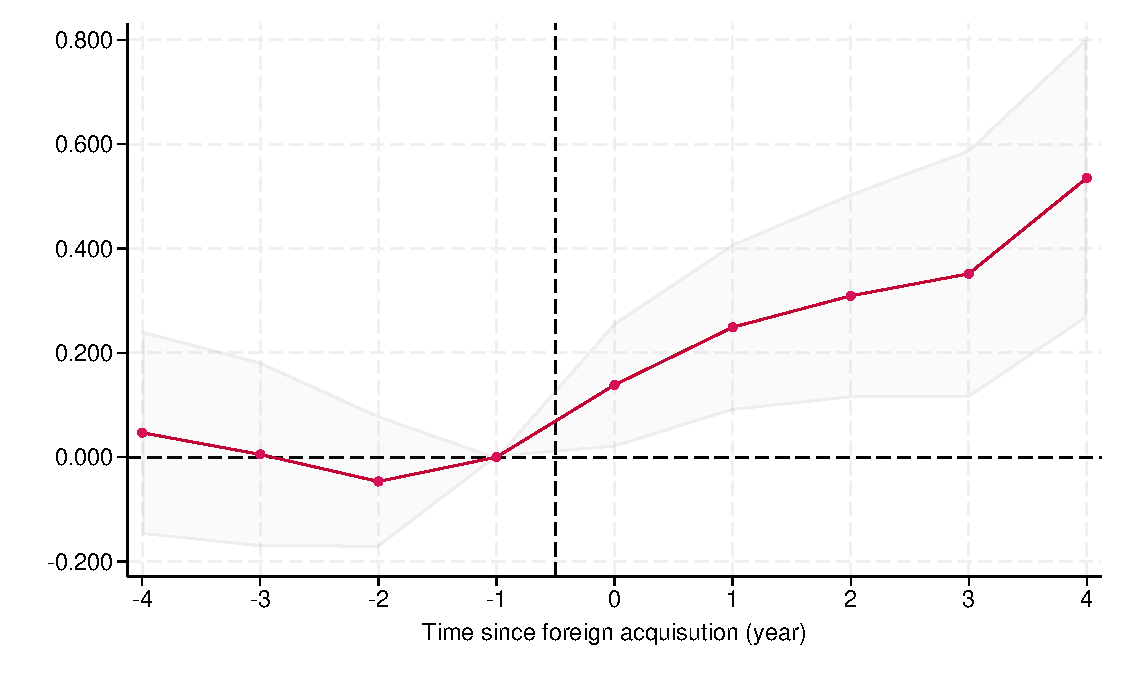
\includegraphics[width=7.5cm]{tab_fig/expat_lnK.pdf}}
    \subfigure[Labor]{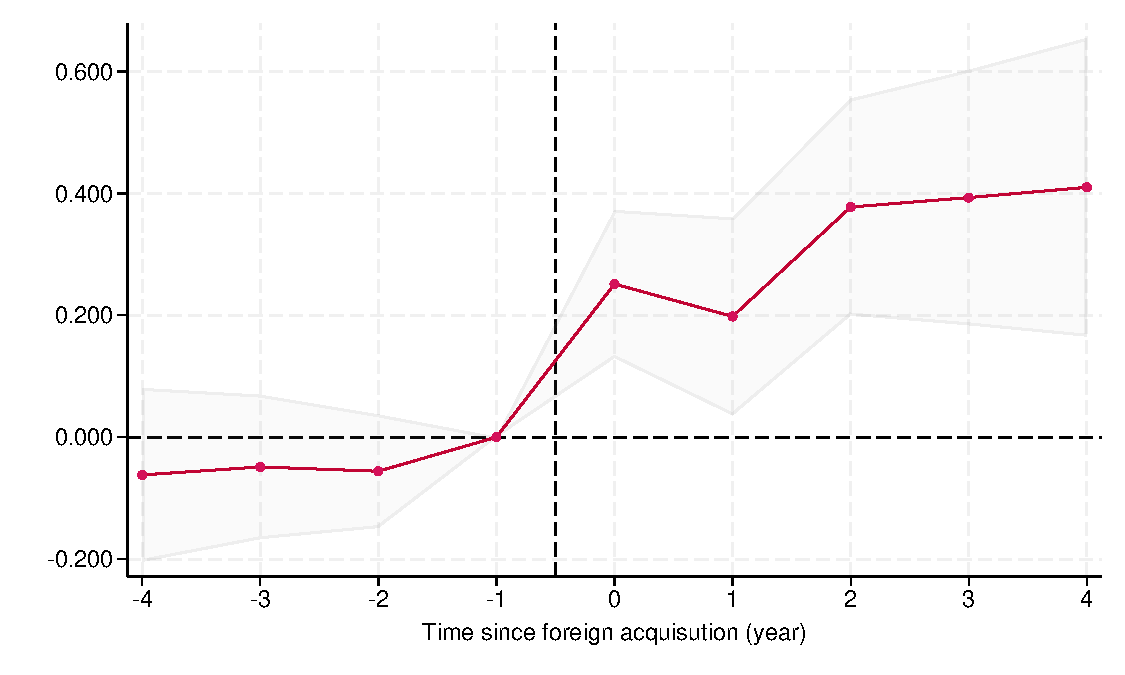
\includegraphics[width=7.5cm]{tab_fig/expat_lnL.pdf}}
    \vspace*{.2cm}
    \subfigure[TFP]{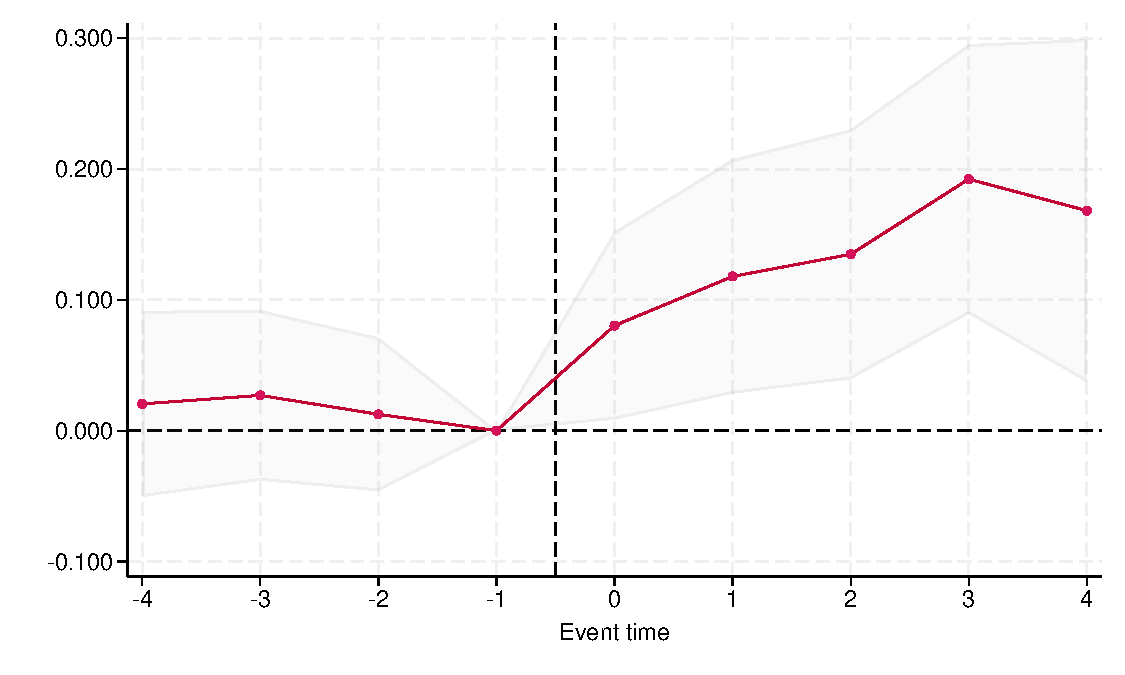
\includegraphics[width=7.5cm]{tab_fig/expat_TFP.pdf}}
    \subfigure[Sales]{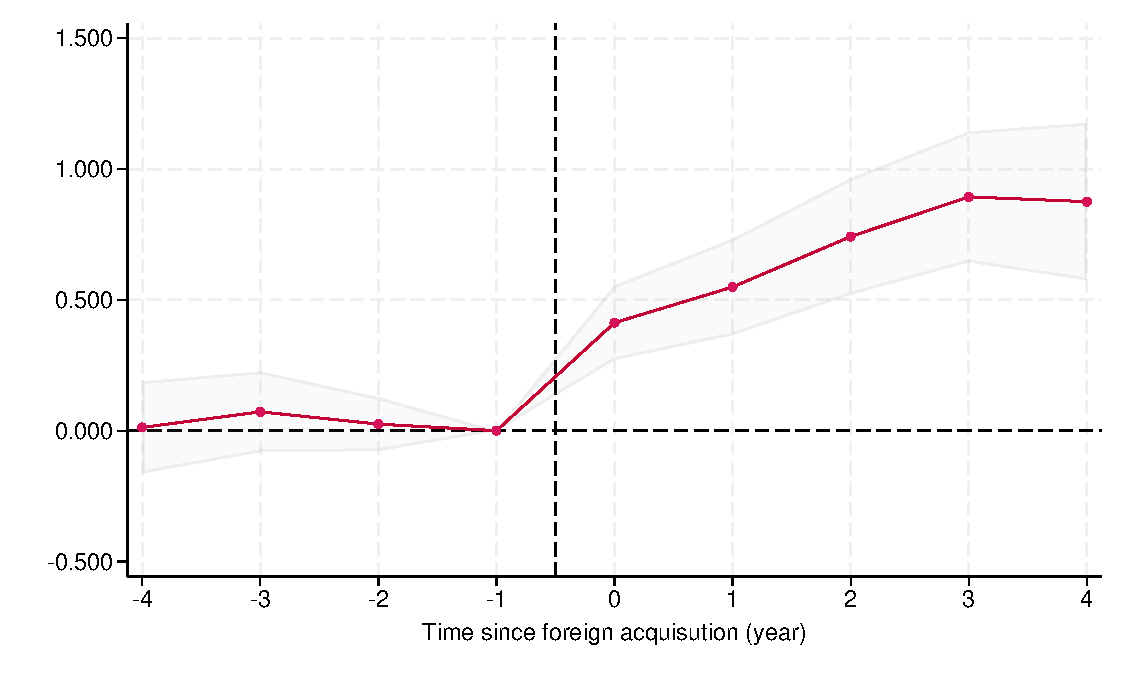
\includegraphics[width=7.5cm]{tab_fig/expat_lnQ.pdf}}
    \vspace*{.2cm}
    \subfigure[Export Share]{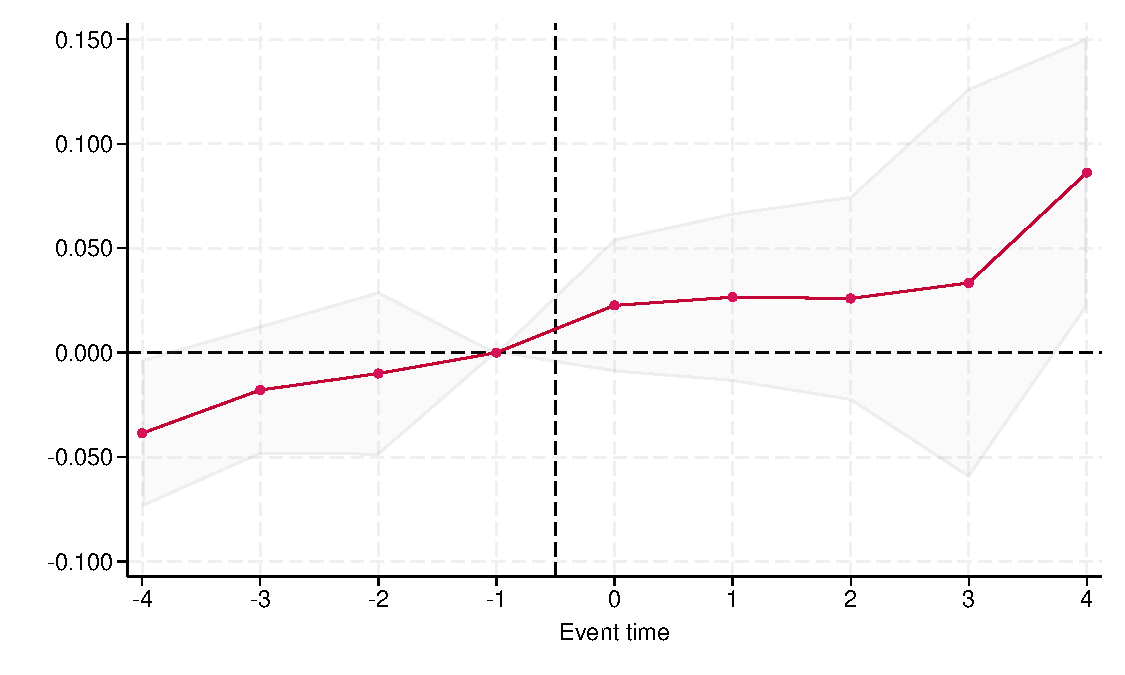
\includegraphics[width=7.5cm]{tab_fig/expat_export_share.pdf}}
    \subfigure[Domestic Sales]{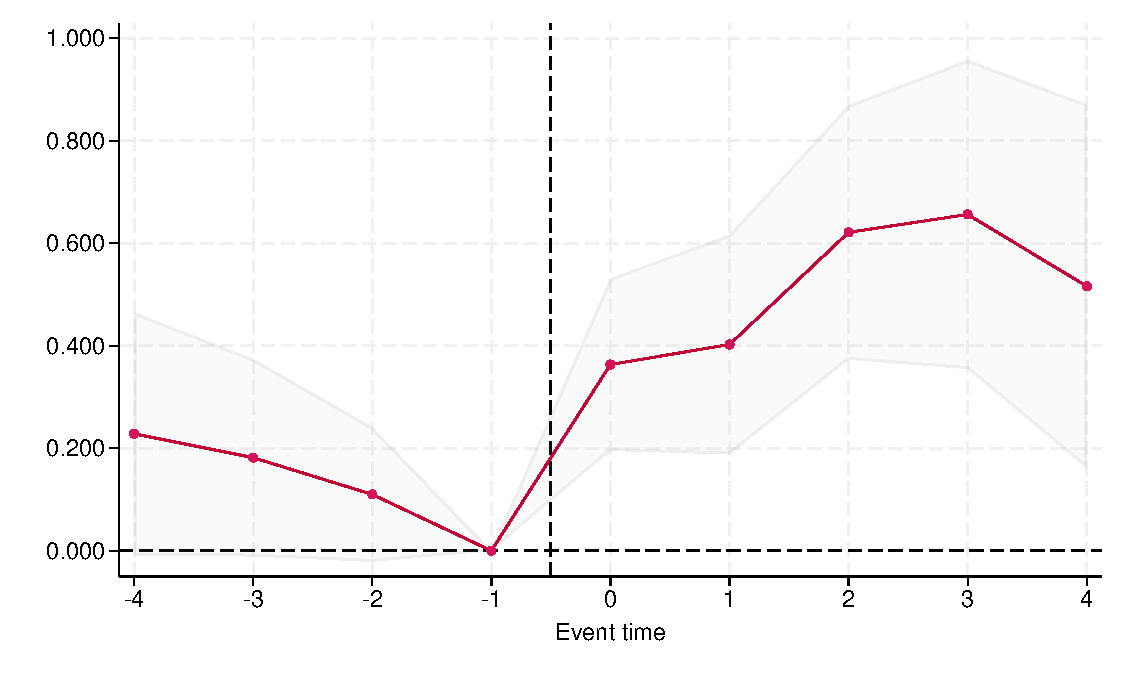
\includegraphics[width=7.5cm]{tab_fig/expat_lnQd.pdf}}
\begin{minipage}{14 cm}
    \caption{Effects of Expatriate CEOs on Firm Outcomes: Event-Time Estimations}
    \label{fig:dynamics}
{Notes: The figures present estimated coefficients and 95-percent confidence intervals of event-time regressions for all firms in the sample. See the notes of Table \ref{tab:effect_ATET}. Coefficients and standard errors are in Appendix Table \ref{tab:dynamics_coeff}.} 
    \end{minipage}    
\end{figure}

\clearpage


\section*{Online Appendix: Additional Figures and Tables}
\vspace*{3 cm}

\setcounter{table}{0}
\renewcommand{\thetable}{A\arabic{table}}
\setcounter{figure}{0}
\renewcommand{\thefigure}{A\arabic{figure}}

    \begin{table}[h!]
    \caption{Shape of the Raw Data}
    \label{table:rawdata}
    \centering
    \begin{tabular}{|l|l|l|l|}
    \hline
    firm & manager & from & to \\
    \hline
    123456 & Bauer Gyöngyi & 1992-01-01 & 1996-12-31 \\
    123456 & Georg Bauer & 1997-01-01 & 1999-12-31 \\
    \hline
    \end{tabular}
     \begin{minipage}{9.5cm}
    \vspace{.2cm}
          \footnotesize {Notes: the table presents two hypothetical entries that identify managerial names and tenures in a given firm as they are in the raw Company Court data. We cannot show actual records to protect the privacy of individuals in the database.}
    \end{minipage}
    \end{table}

\clearpage

\begin{table}[h]
\centering
    \caption{Effects of Expatriate CEOs on Firm Outcomes: Event-Time Estimations. \\  Coefficients and Standard Errors}
    \label{tab:dynamics_coeff}   
   {
\def\sym#1{\ifmmode^{#1}\else\(^{#1}\)\fi}
\begin{tabular}{l*{5}{c}}
\hline\hline
                    &\multicolumn{1}{c}{(1)}&\multicolumn{1}{c}{(2)}&\multicolumn{1}{c}{(3)}&\multicolumn{1}{c}{(4)}&\multicolumn{1}{c}{(5)}\\
                    &\multicolumn{1}{c}{Capital}&\multicolumn{1}{c}{Labor}&\multicolumn{1}{c}{TFP}&\multicolumn{1}{c}{Sales}&\multicolumn{1}{c}{Export Share}\\
\hline
-4                  &       0.045         &      -0.062         &       0.020         &       0.008         &      -0.039\sym{*}  \\
                    &     (0.100)         &     (0.072)         &     (0.036)         &     (0.090)         &     (0.018)         \\
[1em]
-3                  &       0.005         &      -0.049         &       0.027         &       0.072         &      -0.018         \\
                    &     (0.090)         &     (0.060)         &     (0.033)         &     (0.078)         &     (0.016)         \\
[1em]
-2                  &      -0.047         &      -0.056         &       0.013         &       0.025         &      -0.010         \\
                    &     (0.064)         &     (0.047)         &     (0.030)         &     (0.052)         &     (0.020)         \\
[1em]
-1                  &       0.000         &       0.000         &       0.000         &       0.000         &       0.000         \\
                    &         (.)         &         (.)         &         (.)         &         (.)         &         (.)         \\
[1em]
0                   &       0.138\sym{*}  &       0.251\sym{***}&       0.080\sym{*}  &       0.413\sym{***}&       0.023         \\
                    &     (0.061)         &     (0.062)         &     (0.037)         &     (0.072)         &     (0.016)         \\
[1em]
1                   &       0.249\sym{**} &       0.198\sym{*}  &       0.118\sym{**} &       0.549\sym{***}&       0.027         \\
                    &     (0.081)         &     (0.083)         &     (0.046)         &     (0.093)         &     (0.021)         \\
[1em]
2                   &       0.309\sym{**} &       0.378\sym{***}&       0.135\sym{**} &       0.742\sym{***}&       0.026         \\
                    &     (0.099)         &     (0.090)         &     (0.049)         &     (0.113)         &     (0.025)         \\
[1em]
3                   &       0.352\sym{**} &       0.393\sym{***}&       0.192\sym{***}&       0.894\sym{***}&       0.033         \\
                    &     (0.121)         &     (0.107)         &     (0.052)         &     (0.127)         &     (0.048)         \\
[1em]
4                   &       0.535\sym{***}&       0.410\sym{**} &       0.168\sym{*}  &       0.876\sym{***}&       0.086\sym{**} \\
                    &     (0.136)         &     (0.125)         &     (0.067)         &     (0.153)         &     (0.033)         \\
\hline
Observations        &       12714         &       12714         &       12714         &       12714         &       12714         \\
\hline\hline
\end{tabular}
}

  \begin{minipage}{15.5cm}
  \vspace{.2cm}
  \footnotesize {Notes: The table presents the estimated coefficients (standard errors) of two-way fixed effects regressions for all firms in the sample and for industrial and service firms separately. Standard errors clustered at the firm level. Sales are logged, TFP is estimated in one step with capital, labor and material costs as inputs.}
\end{minipage}            
\end{table}


\clearpage

\begin{figure}[h]
    \centering
    \subfigure[Capital]{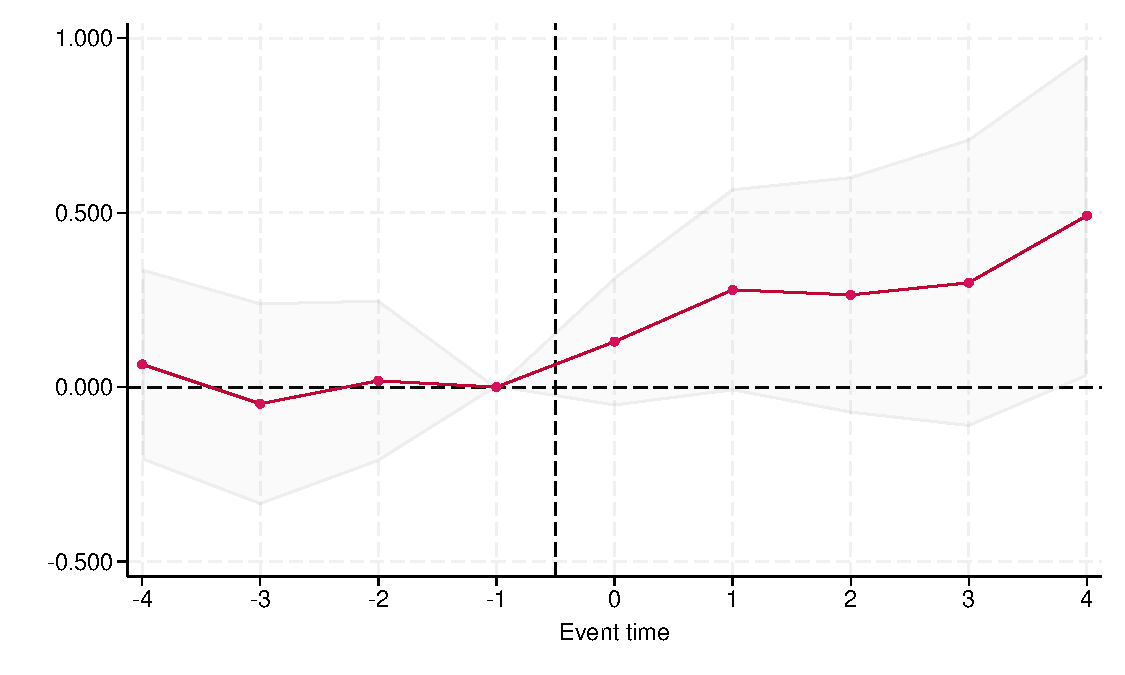
\includegraphics[width=7.5cm]{tab_fig/expat_tradable0_lnK.pdf}}
    \subfigure[Labor]{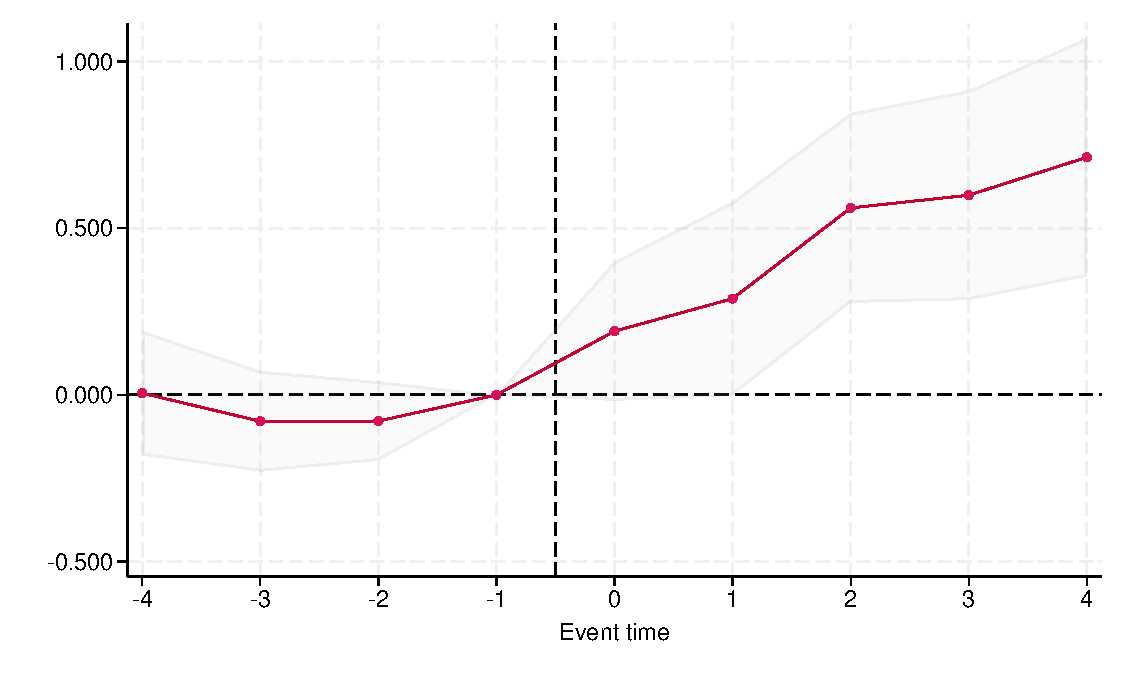
\includegraphics[width=7.5cm]{tab_fig/expat_tradable0_lnL.pdf}}
    \subfigure[TFP]{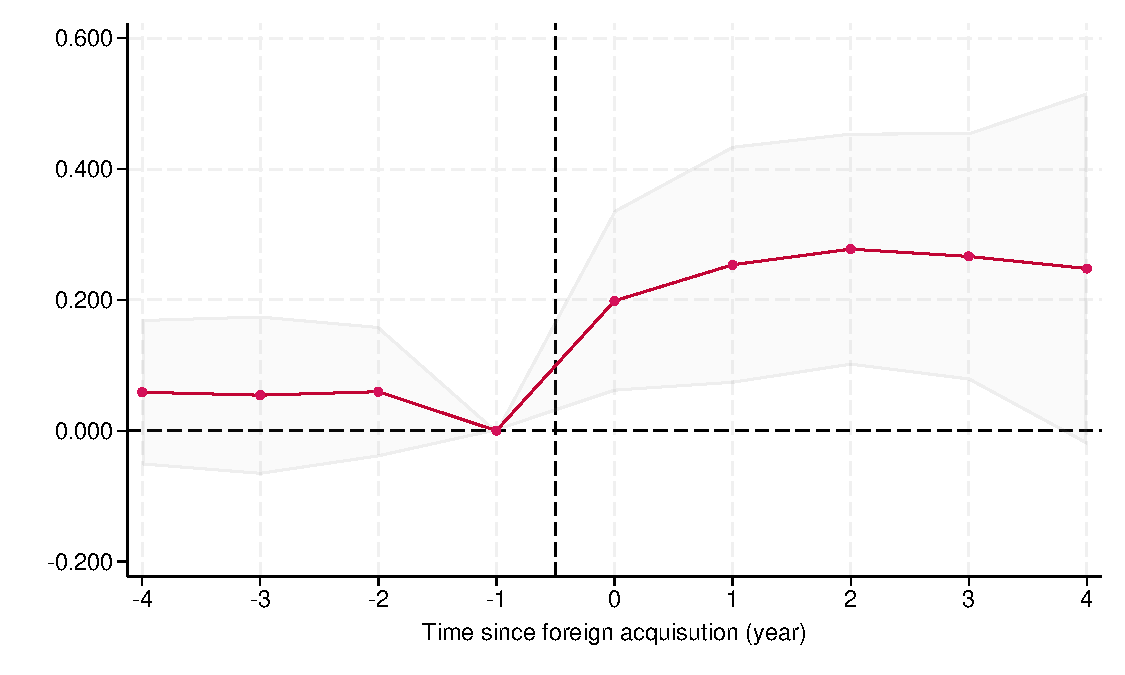
\includegraphics[width=7.5cm]{tab_fig/expat_tradable0_TFP.pdf}}
    \subfigure[Sales]{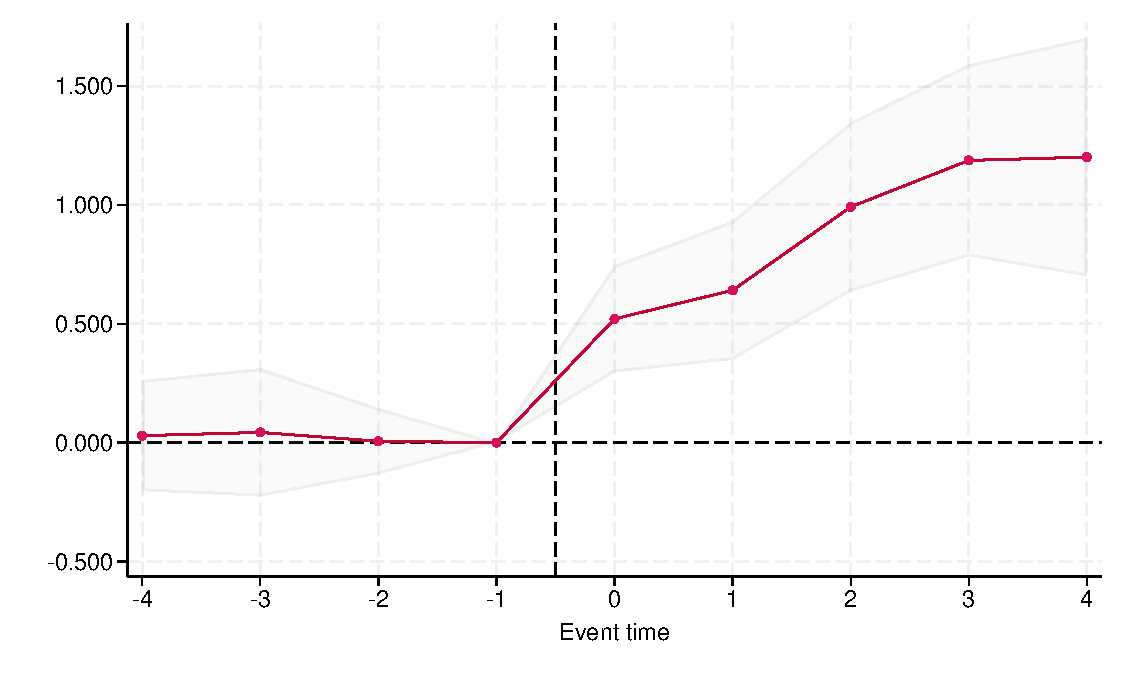
\includegraphics[width=7.5cm]{tab_fig/expat_tradable0_lnQ.pdf}}
    \subfigure[Export Share]{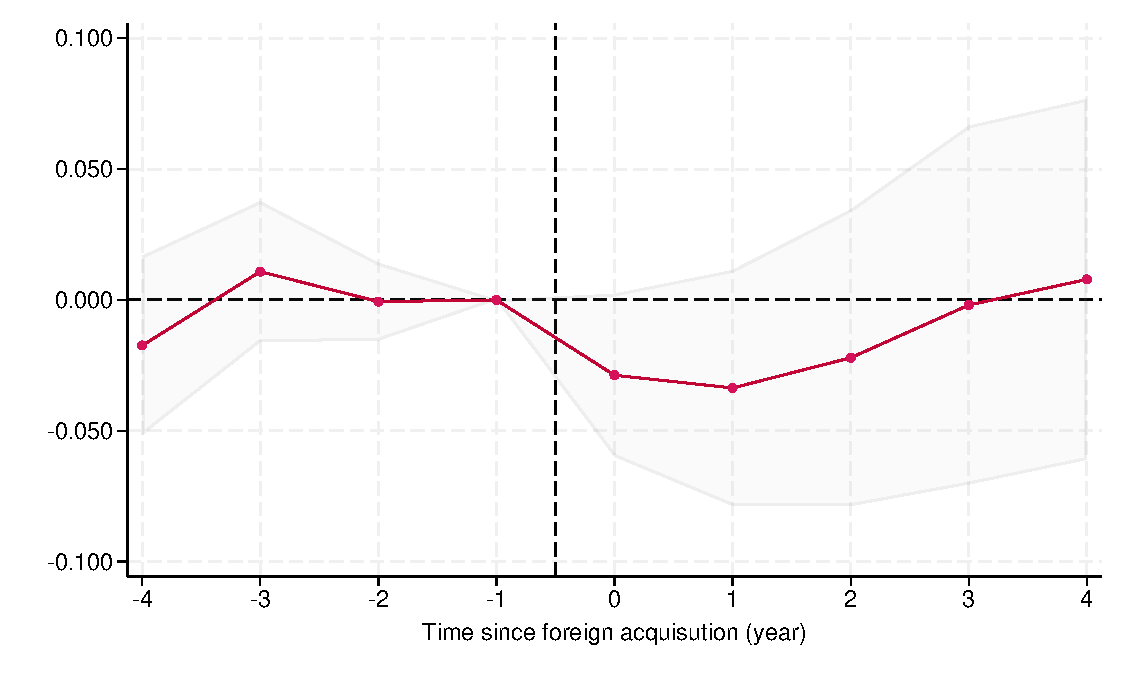
\includegraphics[width=7.5cm]{tab_fig/expat_tradable0_export_share.pdf}}
    \subfigure[Domestic Sales]{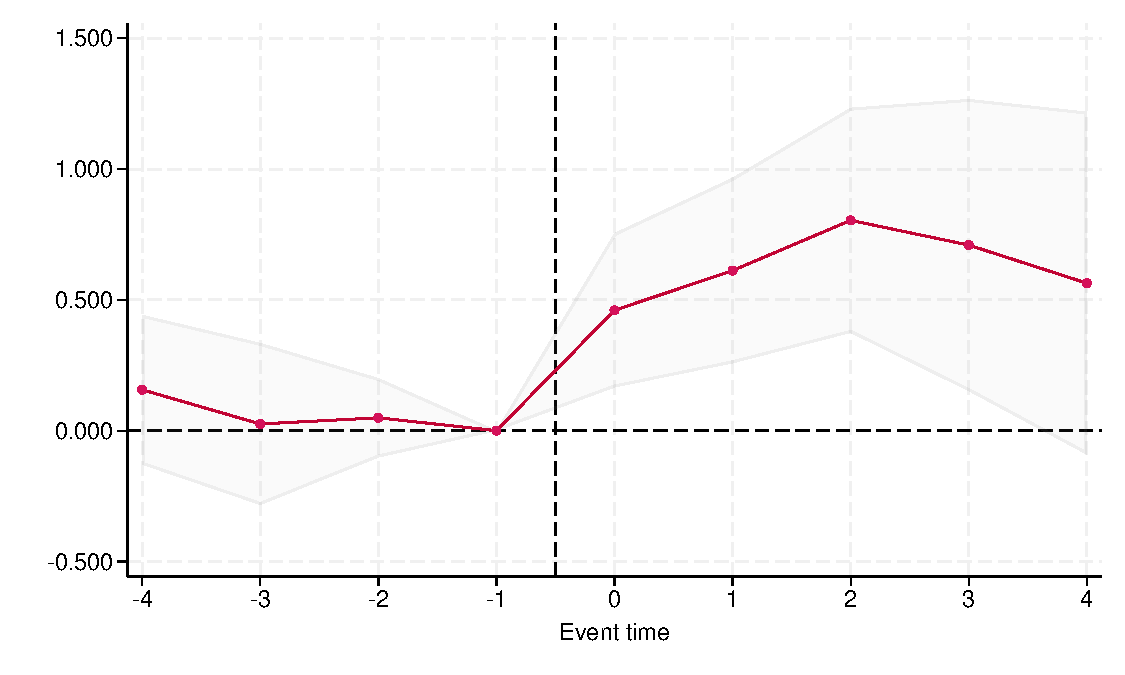
\includegraphics[width=7.5cm]{tab_fig/expat_tradable0_lnQd.pdf}}
\begin{minipage}{14.5 cm}
    \caption{Effects of Expatriate CEOs on Firm Outcomes: Event-Time Estimations. \\ Nontradable Sectors}
   \label{fig:dynamics_nt}
Notes: The figures present estimated coefficients and 95-percent confidence intervals of  event-time regressions for firms in the nontradable sample. See the notes of Table \ref{tab:effect_ATET}. 
    \end{minipage}    
\end{figure}

\begin{figure}[h!]
    \centering
    \subfigure[Capital]{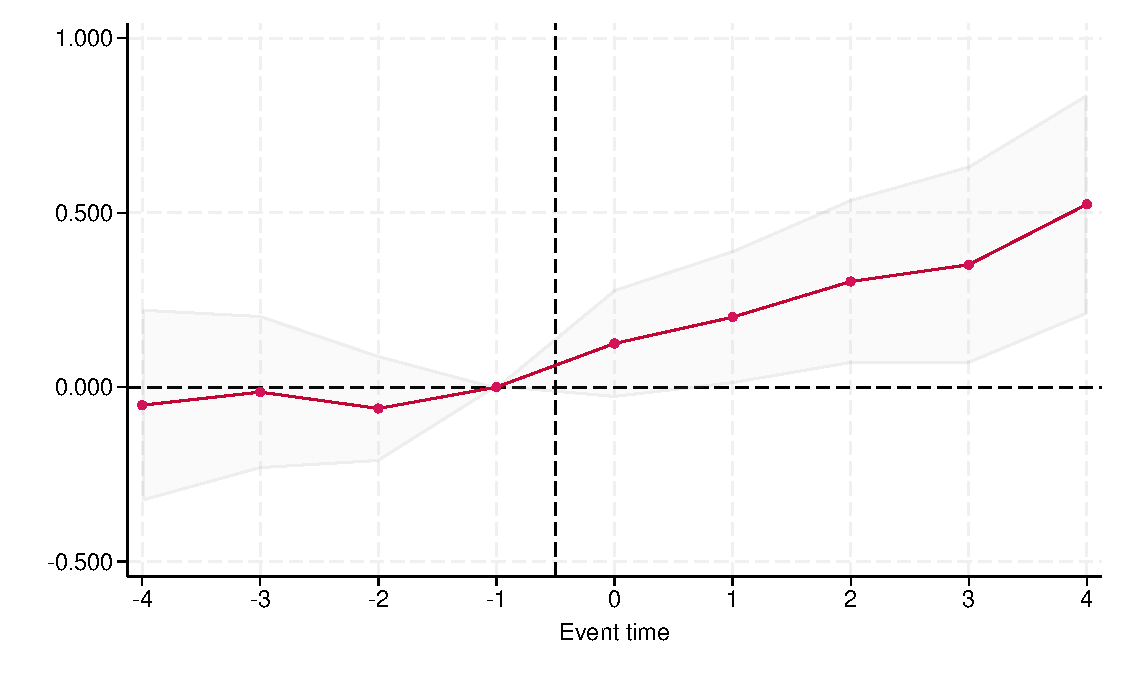
\includegraphics[width=7.5cm]{tab_fig/expat_tradable1_lnK.pdf}}
    \subfigure[Labor]{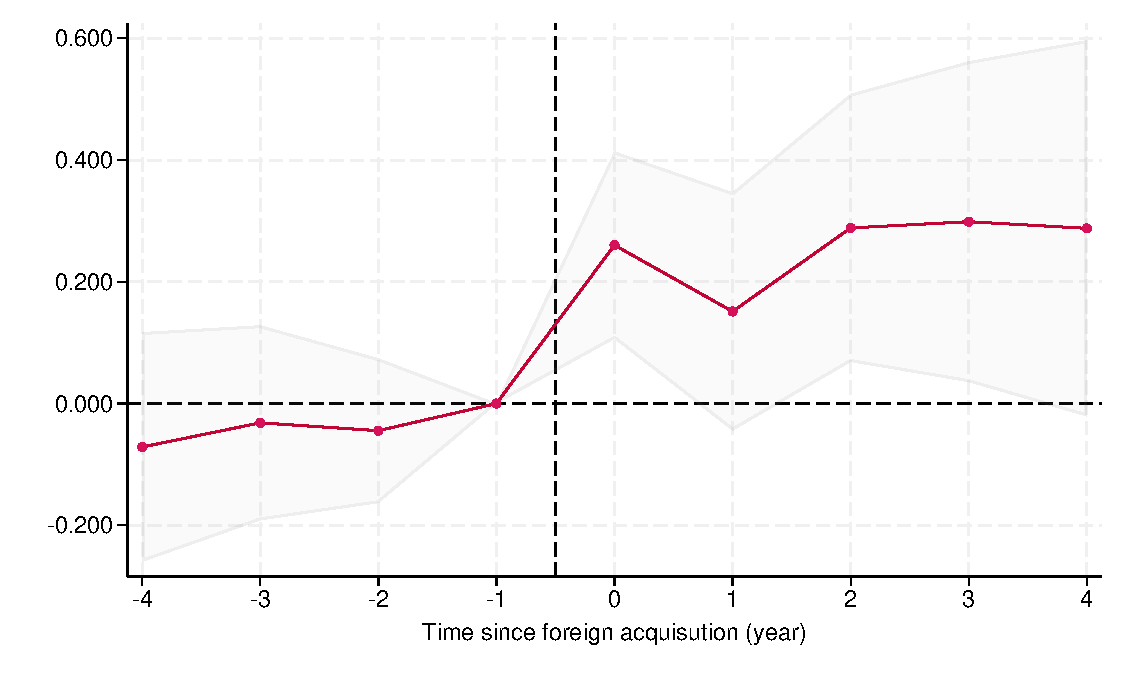
\includegraphics[width=7.5cm]{tab_fig/expat_tradable1_lnL.pdf}}
    \subfigure[TFP]{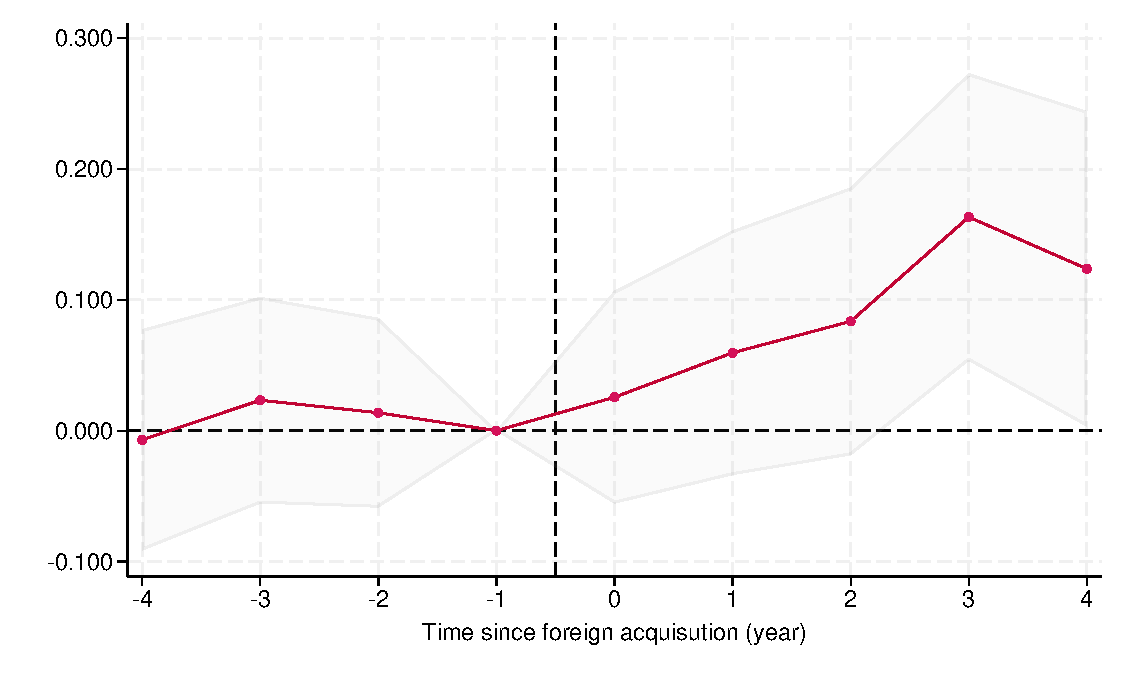
\includegraphics[width=7.5cm]{tab_fig/expat_tradable1_TFP.pdf}}
    \subfigure[Sales]{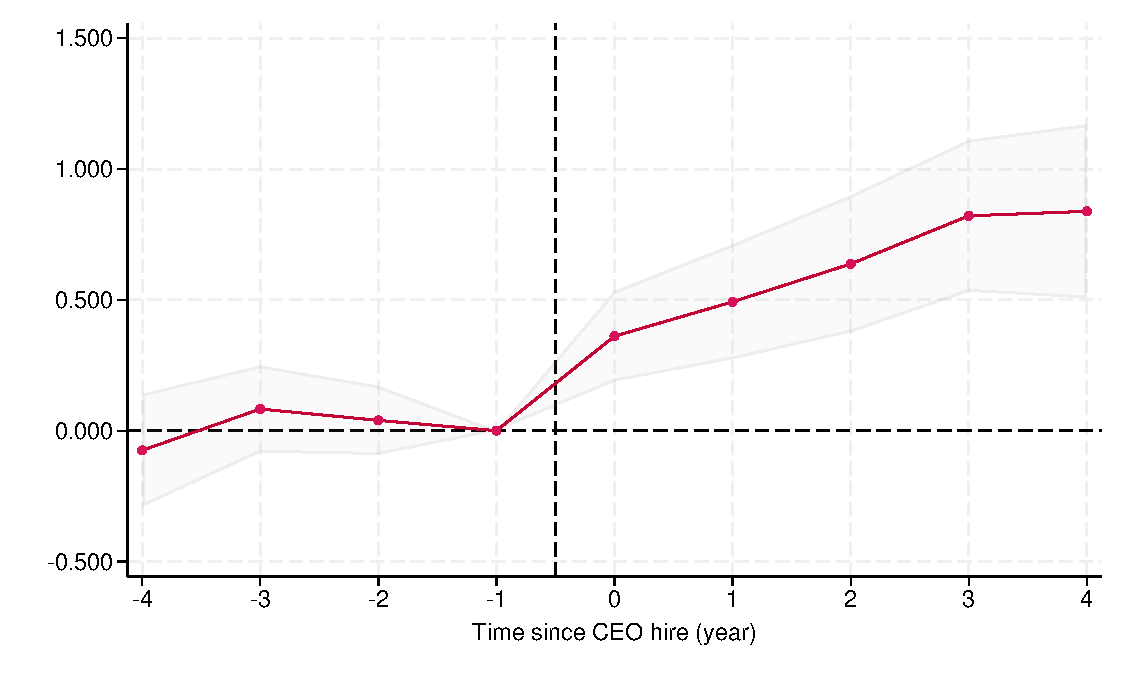
\includegraphics[width=7.5cm]{tab_fig/expat_tradable1_lnQ.pdf}}
    \subfigure[Export Share]{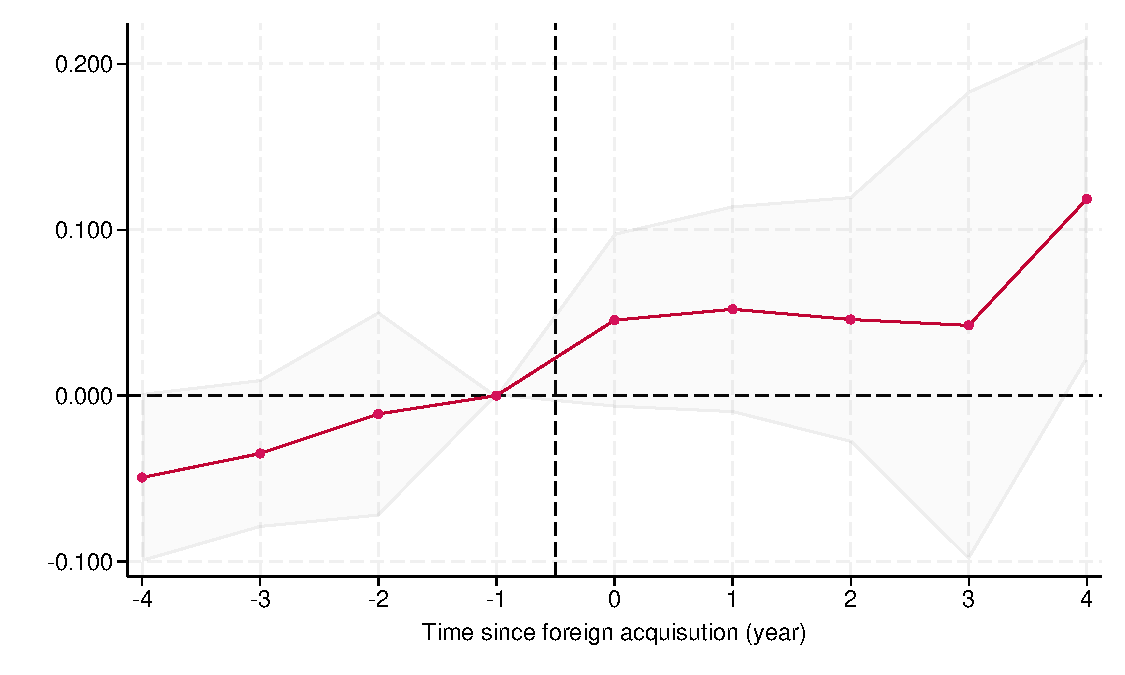
\includegraphics[width=7.5cm]{tab_fig/expat_tradable1_export_share.pdf}}
    \subfigure[Domestic Sales]{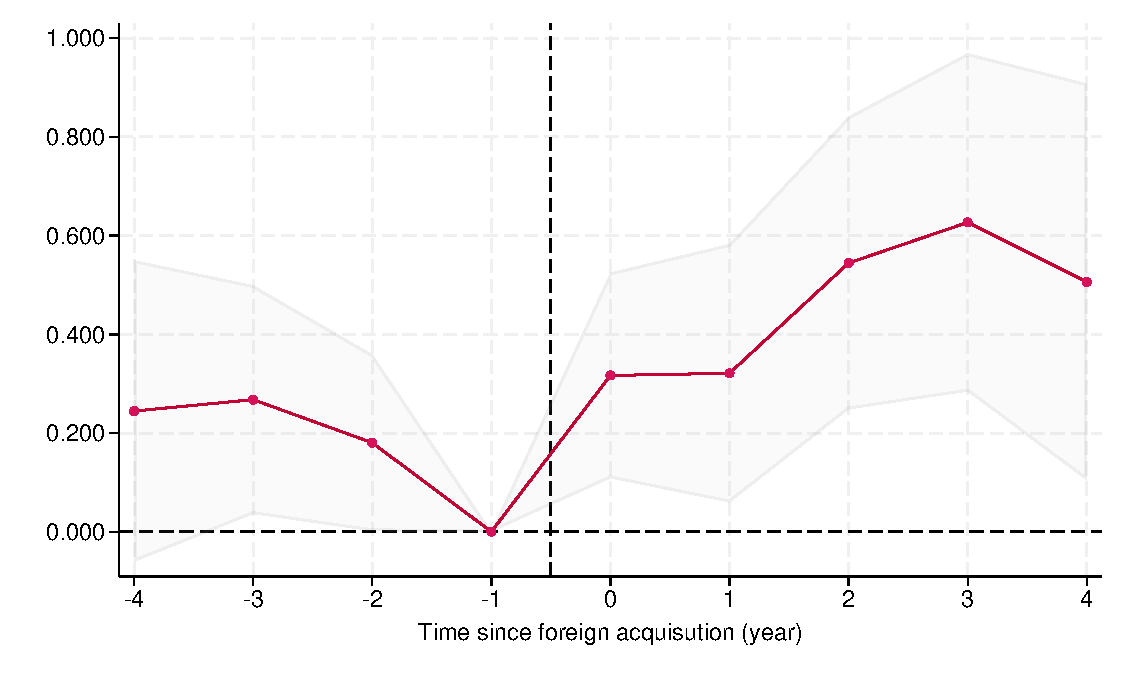
\includegraphics[width=7.5cm]{tab_fig/expat_tradable1_lnQd.pdf}}
\begin{minipage}{14.5 cm}
    \caption{Effects of Expatriate CEOs on Firm Outcomes: Event-Time Estimations. \\ Tradable Sectors}
    \label{fig:dynamics_t}    
Notes: The figures present estimated coefficients and 95-percent confidence intervals of  event-time regressions for firms in the tradable sample. See the notes of Table \ref{tab:effect_ATET}. Coefficients and standard errors are in Appendix Table \ref{tab:dynamics_coeff}.} 
    \end{minipage}    
\end{figure}

\begin{table}[h]
\centering
    \caption{The Effect of Local and Expatriate CEOs on Export Status}
    \label{tab:effect_export}   
   \begin{tabular}{l*{3}{c}}
\hline\hline
                    &\multicolumn{1}{c}{(1)}&\multicolumn{1}{c}{(2)}&\multicolumn{1}{c}{(3)}\\
                    &\multicolumn{1}{c}{Full sample}&\multicolumn{1}{c}{Nontradable}&\multicolumn{1}{c}{Tradable}\\
\hline
Expatriate CEO      &       0.085&       0.068&       0.089\\
                    &     (0.027)&     (0.047)&     (0.033)\\
\hline
Observations        &       12714&        5417&        7297\\
Mean dep.var.       &       0.030&       1.000&       0.000\\
\hline\hline
\end{tabular}

  \begin{minipage}{10.5cm}
  \vspace{.2cm}
  \footnotesize {Notes: The table presents the estimated coefficients (standard errors) of two-way fixed effects regressions for all firms in the sample and for industrial and service firms separately. Standard errors clustered at the firm level. Sales are logged, TFP is estimated in one step with capital, labor and material costs as inputs.}
\end{minipage}            
\end{table}



\end{singlespace}

\end{document}